\section{Introduction} %{{{
\label{s:intro}

% raise issue => 다양한 스토리지가 나옴 => 여전히 fragmentation은 문제가 됨 => 실험이 힘들다..
%-------------------------------------------------------------------------
% conventional SSD를 넘어서 ZNS, OCSSD, KVSSD와 가장 최근에 각광받는 FDP 등 성능과 밀도개선과 함께, 저장장치를 더 스마트하고 능력있게 만드는데 집중하고 있습니다.
% 이런 새로운 유형의 장치들은 저장 장치 환경을 다양화시키고 있습니다. 그에 따라, 새로운 환경에 대한 다양한 연구가 진행되어집니다.
% 예를 들어, ZNS의 경우에는 기존 OS Swap기술의 단점을 해결하고자 하는 연구가 있었습니다.
% 더 이전에 만들어진 저장장치 유형일 수록 더욱 다양한 연구가 진행되어집니다.

% 저장 장치의 성능이 개선됨에 따라 이전에는 큰 문제가 아니였던 fragmentation이 저장 장치 성능에 영향을 미치고 있습니다.
% 새 제품의 저장장치의 성능은 이론적인 성능을 보여줍니다. 하지만, 저장 장치를 사용하면 사용할 수록, 저장장치의 성능이 하락하게 됩니다.
% 이것은 저장장치의 fragmentation 때문입니다.
%-------------
% 이부분은 eval파트로
% Fig[]와 Fig[]은 저장 장치의 사용정도에 따른 latency와 dynamic layout score[]에 대한 그래프입니다.
% Fig[]의 dynamic layout score은 파일 시스템의 단편화 정도를 점수로 나타낸 것입니다. 점수가 낮을 수록 단편화가 더욱 진행된 것입니다.
% 그래프에서 보이는 것과 같이, 장치를 사용하면 사용할 수록 저장장치의 단편화 정도는 커지는 것을 볼 수 있습니다.
% 이와 비례하여 Fig[]에서 보이 듯, latency는 올라가게 됩니다. dynamic layout  score가 수렴함에 따라 latency 또한 수렴하게 됩니다.
% 이런 특징은 F2fs와 ext4 모두에서 같은 양상을 보입니다.
%--------------
% 이러한 이유로, 어떤 저장장치의 유형을 사용하던, 새로운 연구를 진행할 때는 가장 먼저 저장 장치를 노화시켜야 합니다.

% 저장장치를 노화시키기 위한 도구는 여러개가 있습니다.[tbbt:fast05,impressions:fast09,conway:login17]
% 하지만, 노화시키는 과정 중에 live system을 모으는데 많은 시간이 필요하고, Trace들이 매우 크기 때문에 노화에 걸리는 시간은 매우 깁니다.[fs-aging:sigmetrics97]
% Fig[]는 시간에 따른 노화정도입니다. 저장 장치의 크기가 작을 수록 노화되는데 걸리는 시간이 작아지긴 하나, 그럼에도 많은 시간이 요구됩니다.
% 저장장치의 성능과 밀도개선으로 인해, TB단위의 저장장치를 실생활에서 사용하는 만큼, 연구를 위해 노화시키는 시간은 이보다 더욱 많은 시간이 요구될 것입니다.

% 이렇게 낭비되는 시간은, 연구있어서 critical합니다.

Beyond conventional SSDs, new types such as ZNS (Zoned Namespace SSD), OCSSD (Open Channel SSD), KVSSD (Key-Value SSD), and the recently spotlighted FDP (Flexible Data Placement) are focusing on improving performance and density, making storage devices smarter and more capable.
These new types of devices are diversifying the storage environment, leading to various research efforts to explore new conditions.
For example, in the case of ZNS, research has aimed to address the shortcomings of existing OS Swap technology~\cite{znswap}.
As older types of storage devices have been developed, they have prompted numerous research initiatives.

As the performance of storage devices improves, fragmentation, which previously was not a major issue, is now affecting the performance of these devices.
While new products may demonstrate theoretical performance, actual use tends to degrade performance over time due to fragmentation issues.
For this reason, regardless of the type of storage device used, it is imperative to age the storage device first when conducting new research.
\begin{figure}[h]
    \centering
    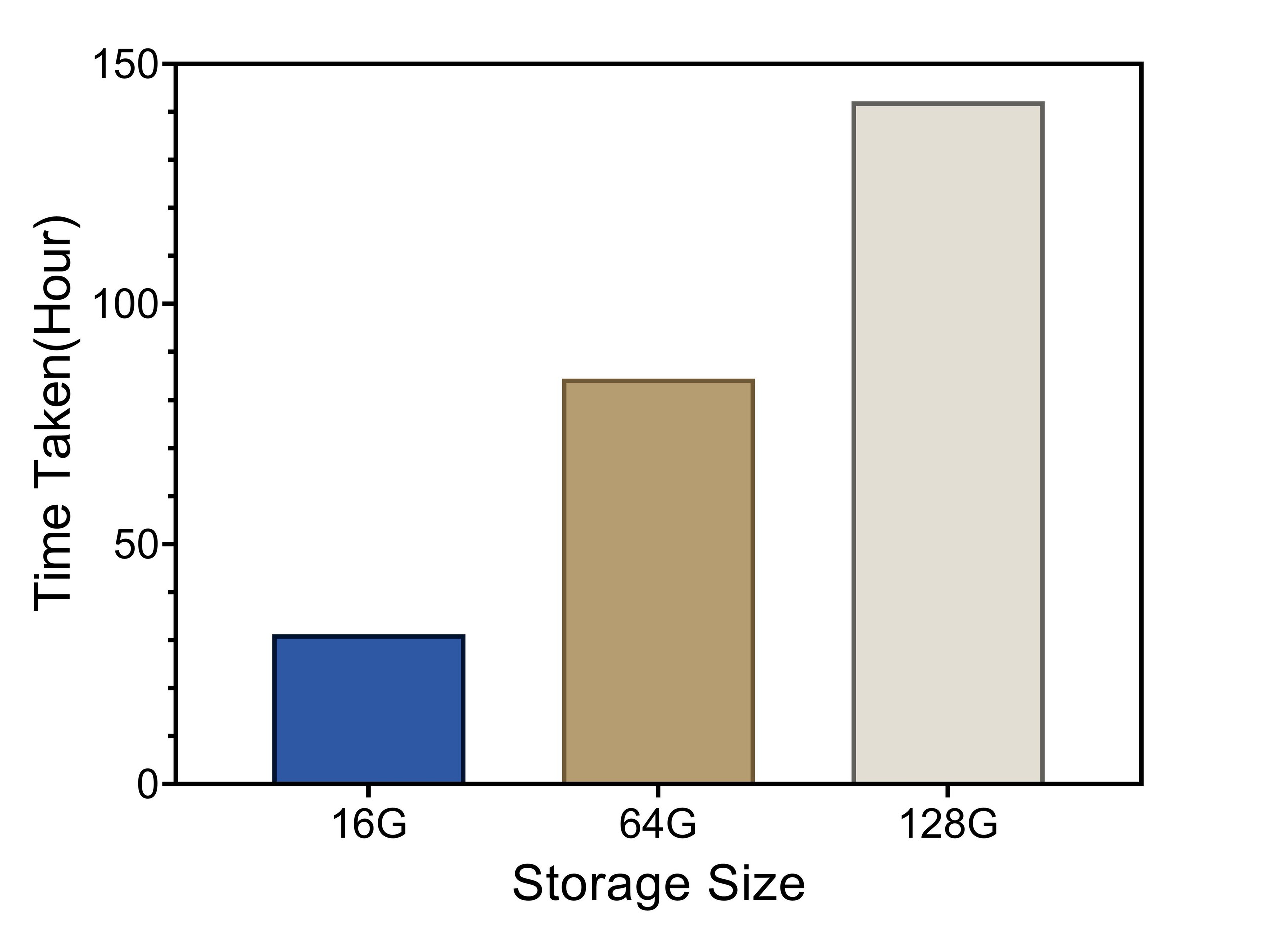
\includegraphics[width=0.95\columnwidth]{graphs/aging_duration}
    \caption{Duration to Aging}
    \label{fig:aging-duration}
\end{figure}
Several tools are available for aging storage devices~\cite{tbbt:fast05, impressions:fast09, conway:login17}.
However, collecting live system data during the aging process is time-consuming, and since the traces are quite large, the duration required for aging is significantly extended \cite{fs-aging:sigmetrics97}.
Figure~\ref{fig:aging-duration} shows the time it takes for storage devices to age. 
Each round takes about 10 minutes, and experiments were conducted using SQLite and the ext4 file system with storage capacities of 16G, 32G, and 128G.
The method for aging is as follows: in each round, small and large files of random sizes are generated randomly. 
All small files are then deleted. If the utilization of the storage remains above a predefined threshold after deleting the small files, it is considered aged~\cite{Problem_in_SSD_Empirical}.
The 64G storage took 2.7 times longer than the 16G storage to age, and the 128G storage took 1.6 times longer than the 64G storage. 
This experiment was conducted in a scenario involving small storage devices, but the smallest 16G storage took 1870 minutes to reach aging. 
This is a considerable amount of time, and in real applications where TB-sized storage devices are used, it would be a tedious wait to reach aging.

Given the performance and density improvements of storage devices, the use of TB-sized storage devices in practical applications will demand even more time for aging for research purposes.

% Goal Setting => snapshot을 만들자 => 단순 복사로는 물리적 조각화를 구현 못함. 논리적 조각화는 많은 반복/ 구성/ 설정이 필요함 => snapshot을 이용하자자
%-------------------------------------------------------------------------
% 낭비되는 시간이 없는 연구활동을 위해 빠른 aging방법이 필요합니다.
% 어떤 aging 시키는 도구를 사용하든 상당한 시간을 사용해야 할것이기 때문에 저희의 요구 사항을 완전히 충족하지 못합니다.
% 또한, 다양한 저장장치에서 노화시키고 싶지만, 저장 장치를 정밀하게 사전 조건화할 적절한 방법이 존재하지 않습니다.
% 따라서, 이와 다른 방법이 필요합니다.
% 이미 aging되어있는 entire storage를 snapshot을 뜨고 사용자에게 제공하면, 사용자는 해당 snapshot을 사용하여 짧은 시간안에 aging된 저장장치를 사용하는 방법을 제안합니다.
% 단순 복사로는 모든 fragmentation을 구현하지 못합니다.
% 2절에서 설명할 physical fragmentation은 논리적 주소 공간과 물리적 주소 공간간의 불일치에서 발생하기 때문입니다.
% 일반적인 SSD에서는 FTL에 접근하기 힘들기 때문에 이와 같은 문제를 재현하기 어렵습니다.

For research activities that do not waste time, a fast aging method is essential.
However, regardless of the aging tool used, it will require significant time, which does not fully meet our requirements.
Additionally, there is currently no appropriate method to precisely precondition storage devices that we want to age.
Therefore, an alternative method is necessary.

We propose providing users with snapshots of the entire storage that has already been aged.
Users can then utilize this snapshot to use the aged storage device within a short time frame.
Simple copying does not adequately replicate all fragmentation.

The physical fragmentation explained in section 2 arises from the mismatch between logical address space and physical address space.
In conventional SSDs, it is challenging to access the FTL (Flash Translation Layer), making it difficult to address such issues.

% Contribution
%-------------------------------------------------------------------------
% 이 논문에서는 aging snapshot인 []을 소개합니다.W
% []은 애뮬레이터를 활용하여 entrie storage를 snapshot을 떠 제공하기 때문에, 빠른 aging된 저장 장치를 사용가능하게 합니다.
% 에뮬레이터인 NVMeVirt를 활용하여 snapshot을 뜨기 때문에 VPN에 대한 정보를 복사할 수 있습니다.
% 그리고, FTL도 그대로 복사할 수 있어 physical fragmentation에 대한 문제도 해결할 수 있게 됩니다.
% 추가적으로, 우리가 제공할 snapshot을 사용자가 쉽게 다루기 위해, snapshot의 크기를 줄이는 능력도 가지고 있습니다.
% 사용자는 다양한 저장장치에서 다양한 조건에 맞는 snapshot을 가지고 빠른 aging된 저장장치를 구성할 수 있습니다.
% 따라서, [] 기술은 연구 활동에서 aging에 걸리는 시간을 없애주어, 혁신적인 저장 장치 개발을 촉진합니다.
In this paper, we introduce the aging snapshot method, [].
This method allows for the utilization of an entire storage snapshot, enabling the use of fast-aged storage devices.
By employing the emulator NVMeVirt to create snapshots, we can also replicate information related to the VPN (Virtual Physical Number).
Additionally, by copying the FTL (Flash Translation Layer) as well, we can address the issue of physical fragmentation.

Furthermore, to assist users in handling the snapshots we provide, we have the capability to reduce the size of the snapshots.
Users can build fast-aged storage devices tailored to various conditions with different snapshots from various storage devices.
Thus, the [] technology eliminates the time spent in aging during research activities, promoting the innovative development of storage devices.

% Paper Progress => 이부분...
